\documentclass[xcolor=svgnames,dvipsnames,table, hyperref=pdftex, mathserif, presentation]{beamer}
\usepackage{amsmath,amssymb,amsfonts,amsthm}
\usepackage{ctex}
\usepackage{graphics}
\usepackage{graphicx}
\usepackage{xcolor}
\usepackage{wasysym}
\usepackage{bbm}
\usepackage{url}
\usepackage{beamerleanprogress}
\usepackage{tikz-dependency}
\usepackage{tikz-qtree}

\usetheme{CambridgeUS}
%\usetheme{Pittsburgh}
\usecolortheme{orchid} % seahorse  orchid rose
\setbeamertemplate{blocks}[rounded][shadow=true]
\AtBeginSection[]{%
  \begin{frame}<beamer>
    \frametitle{Outline}
      \tableofcontents[current] 
    \end{frame}
  \addtocounter{framenumber}{-1}% If you don't want them to affect the slide number
}
\AtBeginSubsection[]
{
  \begin{frame}
  \frametitle{Outline}
    \tableofcontents[currentsection,currentsubsection]
  %\tableofcontents[sectionstyle=show/hide,subsectionstyle=hide/show/hide]
  \end{frame}
  \addtocounter{framenumber}{-1}% If you don't want them to affect the slide number
}
\newcommand{\setof}[1]{\ensuremath{\left \{ #1 \right \}}}
\newcommand{\tuple}[1]{\ensuremath{\left \langle #1 \right \rangle }}
\newcommand{\red}[1]{\textcolor{red}{#1}}
\newcommand{\brown}[1]{\textcolor{brown}{#1}}
\newcommand{\green}[1]{\textcolor{green}{#1}}
\newcommand{\blue}[1]{\textcolor{blue}{#1}}
\newcommand{\cyan}[1]{\textcolor{cyan}{#1}}

%gets rid of navigation symbols
\setbeamertemplate{navigation symbols}{}

\begin{document}

\title[Paraphrase]{Dynamic Pooling and Unfolding Recursive Autoencoders for Paraphrase Detection (NIPS2011)}

\institute[icst@pku]{
  
}
\author[Zhe Han]{\\ Zhe Han \\ 1401214342\\ iampkuhz@gmail.com
}

\frame[t,plain]{ \titlepage } % [t,plain]

\frame{
  \frametitle{ Outline  }
  
   \begin{itemize}
  \item Paraphrase identification(复述检测)
    \begin{itemize}
     \item Definition
     \item Common methods
    \end{itemize}

  \item 本文的方法
    \begin{itemize}
      \item Recursive Autoencoder
      \item Dynamic Pooling
      \item Experiment Result
    \end{itemize}

  \item 实验效果
    \begin{itemize}
    \item 分析, 对比其他任务
    \end{itemize}
  \end{itemize}

}

\frame{
  \frametitle{Paraphrase identification}
  
  \begin{itemize}
   \item definition
      \begin{itemize}
       \item 给定一组句子, 判断其是否是复述
	  \begin{itemize}
	   \item binary classification
	  \end{itemize}

      \end{itemize}
      
    \item Microsoft Research Paraphrase Corpus (MSRP)
	\begin{itemize}
	 \item train: 4,076 sentence pairs (2,753 positive: 67.5 \%)
	 \item test: 1,725 sentence pairs (1,147 positive: 66.5 \%)
	 \item 2个标注者, 83\%的一致性, 第三个人更正
	\begin{block}{Sample data}
	 \begin{itemize}
	 	 \item Sentence 1: Amrozi accused his brother, whom he called "the witness", of deliberately distorting his evidence.
	       \item Sentence 2: Referring to him as only "the witness", Amrozi accused his brother of deliberately distorting his evidence.
	       \item Class: 1 (true paraphrase)
	 \end{itemize}
	\end{block}
	
	\end{itemize}
  \end{itemize}

}


\frame{
    \frametitle{Paraphrase identification}
    \begin{itemize}
     \item Common methods
	\begin{itemize}
	  \item lexical features
	      \begin{itemize}
	       \item n-gram features, skip-gram fatures, ...
	      \end{itemize}

	  \item semantic features
	      \begin{itemize}
	       \item POS tag, wordnet similarity, dependency tree relation, ...
	      \end{itemize}

	  \item classification
	      \begin{itemize}
	       \item SVM, voted classifications
	      \end{itemize}
	\end{itemize}
    
    \item Challenge
	\begin{itemize}
	 \item 没有提取句子的全局信息( dependency features利用不足)
	 \item 对句子涵义的特征提取不足(没有真正理解句子)
	\end{itemize}

    \end{itemize}

}

\frame{
    \frametitle{This paper}
    \begin{block}{Main method}
	\begin{itemize}
	 \item 利用NYT新闻训练每个单词的向量(100维)
	 \item 对于每个句子(多个单词向量)采用训练一个递归的自动编码机, 得到一个句子级别的语义向量. 
	 \item 通过判断两个句子的语义向量的相似性得到语义相似性特征
	\end{itemize}
    \end{block}

    \begin{itemize}
	 \item 递归的自动编码机(Unfolding Recursive Autoencoder) 
	    \begin{itemize}
	     \item 抽取句子的语义向量, 得到语法数上每个节点(单词, 短语)的向量
	    \end{itemize}
	 \item Dynamic Pooling
	    \begin{itemize}
	     \item 对于长度变化的两个句子, 抽取固定维数的特征
	    \end{itemize}

	\end{itemize}

}

\frame{
     \frametitle{Unfolding Recursive Autoencoder}
  \begin{figure}[h]
  \centering
  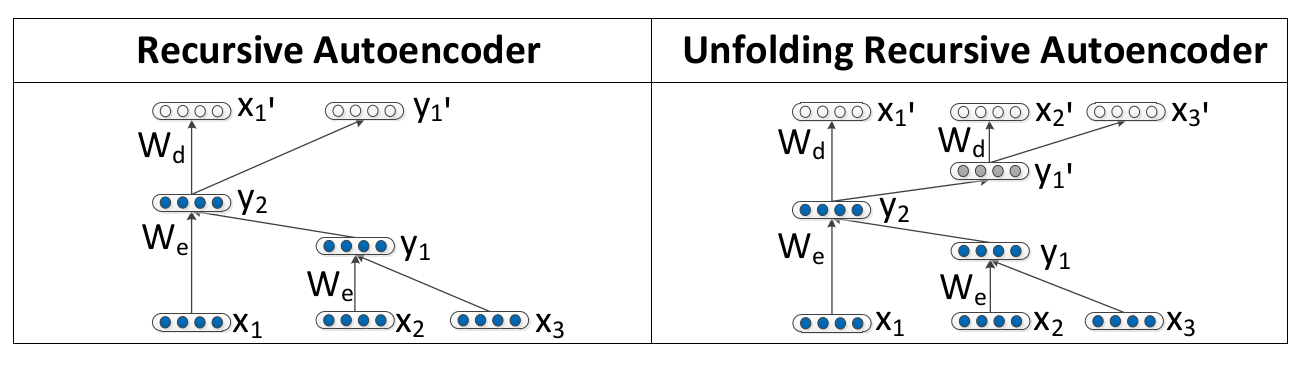
\includegraphics[width=0.8\textwidth]{uRAE}
  \end{figure}
  
  \begin{itemize}
      \item Comparison (on $y_2 -> x_1y_1$)
	  \begin{itemize}
	   \item Autoencoder
	      \begin{itemize}
	       \item minimum $\parallel y_2'-y_2\parallel$
	      \end{itemize}
	
	   \item Recursive Autoencoder
	   \begin{itemize}
	    \item minimum $\parallel[x_1';y_1']-[x_1;y_1]\parallel $
	   \end{itemize}
 
	   \item Unfolding Recursive Autoencoder
	      \begin{itemize}
	       \item  minimum $\parallel[x_1';x_2';...;x_j']-[x_1;x_2;...;x_j]\parallel $
	      \end{itemize}
	  \end{itemize}
      
    \end{itemize}
}

\frame{
    \frametitle{Unfolding Recursive Autoencoder(RAE)}
    \begin{itemize}
     \item u RAE 和 RAE类似, 我们通过解释RAE来说明
    \end{itemize}

}

\end{document}
